% Diagram architektúry spracovania v module NOISE (zdrojový tvar obrázka).
% Preklad: pdflatex architektura.tex  ->  architektura.pdf (vkladá sa do článku)
\documentclass[tikz,border=4pt]{standalone}
\usepackage[T1]{fontenc}
\usepackage[utf8]{inputenc}
\usepackage{mathptmx}
\usetikzlibrary{positioning,arrows.meta,fit,backgrounds}

\begin{document}
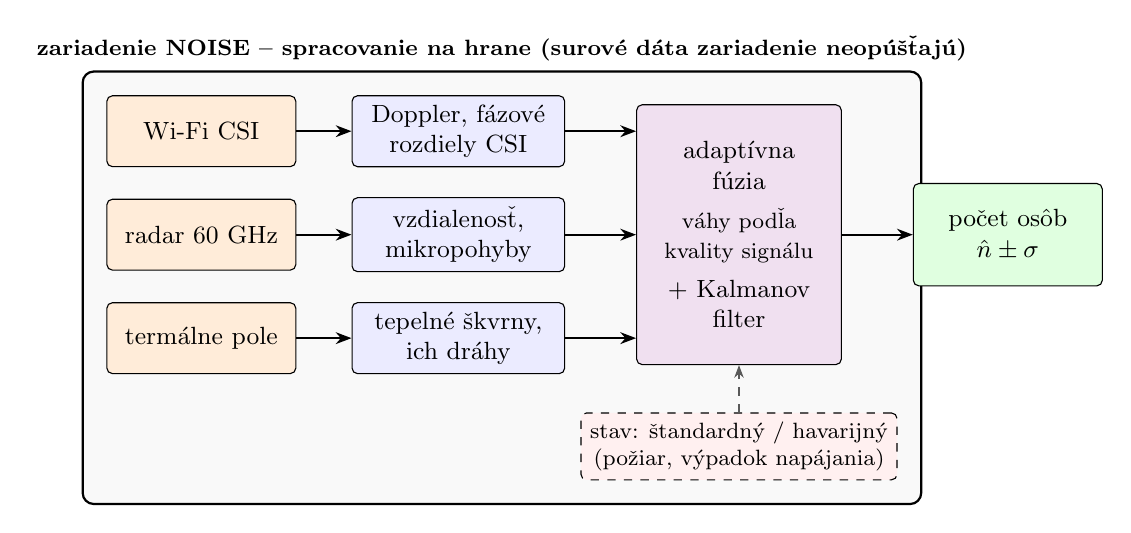
\begin{tikzpicture}[
  font=\small,
  node distance=4mm and 7mm,
  sen/.style={draw, rounded corners=2pt, fill=orange!15, minimum width=24mm, minimum height=9mm, align=center},
  blk/.style={draw, rounded corners=2pt, fill=blue!8, minimum width=27mm, minimum height=9mm, align=center},
  fus/.style={draw, rounded corners=2pt, fill=violet!12, minimum width=26mm, minimum height=33mm, align=center},
  vys/.style={draw, rounded corners=2pt, fill=green!12, minimum width=24mm, minimum height=13mm, align=center},
  ar/.style={-{Stealth[length=2mm]}, thick},
  q/.style={-{Stealth[length=1.6mm]}, dashed, gray!70!black}
]
% senzory
\node[sen] (csi) {Wi-Fi CSI};
\node[sen, below=of csi] (rad) {radar 60 GHz};
\node[sen, below=of rad] (ir) {termálne pole};

% extrakcia príznakov
\node[blk, right=of csi] (f1) {Doppler, fázové\\rozdiely CSI};
\node[blk, right=of rad] (f2) {vzdialenosť,\\mikropohyby};
\node[blk, right=of ir]  (f3) {tepelné škvrny,\\ich dráhy};

% fúzia
\node[fus, right=9mm of f2] (fu) {adaptívna\\fúzia\\[3pt]{\footnotesize váhy podľa}\\{\footnotesize kvality signálu}\\[3pt]+ Kalmanov\\filter};

% výstup
\node[vys, right=9mm of fu] (vy) {počet osôb\\$\hat{n} \pm \sigma$};

\draw[ar] (csi) -- (f1);
\draw[ar] (rad) -- (f2);
\draw[ar] (ir)  -- (f3);
\draw[ar] (f1.east) -- (fu.west |- f1.east);
\draw[ar] (f2.east) -- (fu.west |- f2.east);
\draw[ar] (f3.east) -- (fu.west |- f3.east);
\draw[ar] (fu) -- (vy);

% režim
\node[draw, dashed, rounded corners=2pt, below=6mm of fu, align=center, font=\footnotesize, fill=red!6] (rez)
  {stav: štandardný / havarijný\\(požiar, výpadok napájania)};
\draw[q] (rez) -- (fu);

% hranica zariadenia
\begin{scope}[on background layer]
\node[draw, thick, rounded corners=4pt, fill=gray!5, inner sep=3mm, fit=(csi)(ir)(f1)(f3)(fu)(rez),
      label={[font=\footnotesize\bfseries]above:zariadenie NOISE -- spracovanie na hrane (surové dáta zariadenie neopúšťajú)}] (dev) {};
\end{scope}
\end{tikzpicture}
\end{document}
